\documentclass[10pt]{extarticle}
\usepackage[a4paper,margin=1.5cm,columnsep=0.7cm]{geometry}
\usepackage{amsmath,amssymb}
\usepackage{graphicx}
\usepackage{enumitem}
\usepackage{booktabs}
\usepackage{array}
\usepackage{tabularx}
\usepackage[T1]{fontenc}
\usepackage{multicol}

\setlength{\parindent}{0pt}
\setlength{\parskip}{4pt}
\renewcommand{\arraystretch}{1.15}

\newenvironment{qoptions}{\begin{itemize}[leftmargin=1.8em,itemsep=2pt,topsep=2pt,label={}]}{\end{itemize}}
\newcommand{\opt}[2]{\item[({#1})] {#2}}

\newcommand{\sectionhdr}[1]{\par\vspace{4pt}\noindent\textbf{\large #1}\par\vspace{2pt}}
\newcommand{\subsectionhdr}[1]{\par\vspace{3pt}\noindent\textbf{#1}\par\vspace{2pt}}

\pagestyle{empty}

\begin{document}
\begin{center}
{\LARGE\bfseries JEE (Main+Advanced) Score-II --- Test 44 (23 Mar 2025)}
\end{center}
\vspace{6pt}

\begin{multicols}{2}

\sectionhdr{PART-1: PHYSICS}
\subsectionhdr{Section-I (i): Single Correct}

\textbf{1.} A thin uniform rod of mass m lies on a horizontal table. Find minimum horizontal force that should be applied to the end of the rod perpendicular to it so that, it can be moved. (Coefficient of friction is $\mu$)

\begin{center}
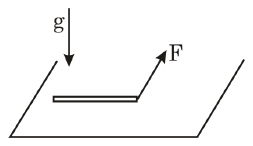
\includegraphics[width=0.55\linewidth]{Score-II - Test 44 (23 Mar 2025)-img/p1phy_q1_rod.png}
\end{center}

\begin{qoptions}
\opt{A}{$\mu mg$}
\opt{B}{$\dfrac{\mu mg}{\sqrt2}$}
\opt{C}{$(\sqrt2-1)\mu mg$}
\opt{D}{$\left(1-\dfrac1{\sqrt2}\right)\mu mg$}
\end{qoptions}

\textbf{2.} Consider a planar conducting frame rotating at a constant angular velocity in a uniform magnetic field. The frame is made of thin rigid wires with same uniform curvature and same resistance per unit length. What fraction of the total heat released is released by the outermost wires?

\begin{center}
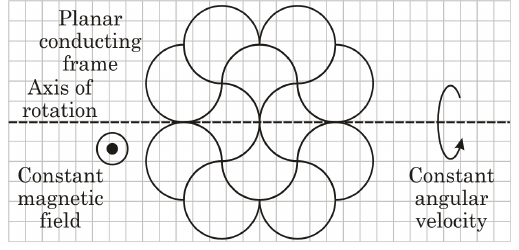
\includegraphics[width=0.85\linewidth]{Score-II - Test 44 (23 Mar 2025)-img/p1phy_q2_frame.png}
\end{center}

\begin{qoptions}
\opt{A}{0.33}
\opt{B}{0.72}
\opt{C}{0.86}
\opt{D}{None of these}
\end{qoptions}

\textbf{3.} The bottom face of a regular tetrahedron with edge a, completely immersed in a liquid of density $\rho$, is at depth h. Determine the net force exerted by the liquid on the side edges of the tetrahedron. (Neglect atmospheric pressure)

\begin{center}
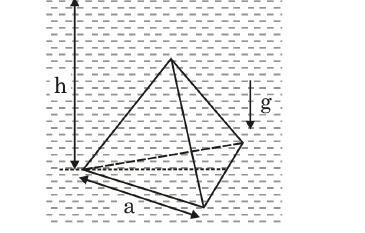
\includegraphics[width=0.55\linewidth]{Score-II - Test 44 (23 Mar 2025)-img/p1phy_q3_tetrahedron.png}
\end{center}

\begin{qoptions}
\opt{A}{$F=\dfrac1{12}\rho ga^2\left(3\sqrt3h-\sqrt2a\right)$}
\opt{B}{$F=\dfrac{\rho ga^2}{24}\left(3\sqrt3h-\sqrt2a\right)$}
\opt{C}{$F=\dfrac{\rho ga^2}6\left(\sqrt3h-\sqrt2a\right)$}
\opt{D}{None of these}
\end{qoptions}

\textbf{4.} A bowl of height $\dfrac{4r}3$ is formed by removing the top third of a sphere (of radius r). A small marble of mass m rests at the bottom of the bowl. Assuming all surfaces are frictionless and ignoring air resistance, find the maximum initial velocity that could be given to the marble for it to land back in the bowl.

\begin{center}
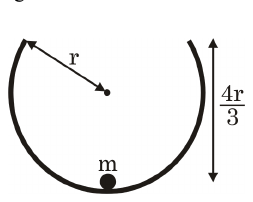
\includegraphics[width=0.55\linewidth]{Score-II - Test 44 (23 Mar 2025)-img/p1phy_q4_bowl.png}
\end{center}

\begin{qoptions}
\opt{A}{$\sqrt{\dfrac{14gr}3}$}
\opt{B}{$\sqrt{\dfrac{16gr}3}$}
\opt{C}{$\sqrt{\dfrac{17gr}3}$}
\opt{D}{$\sqrt{\dfrac{19gr}3}$}
\end{qoptions}

\subsectionhdr{Section-I (ii): One or more correct}

\textbf{5.} A uniform thin rigid rod of mass m is supported by two rapidly rotating rollers, whose axes are separated by a fixed distance a. The rod is initially placed at rest symmetrically as shown in Fig.1. Assume that the rollers rotate in opposite directions as shown in fig.1. The coefficient of kinetic friction between the rod and the rollers is $\mu$. Now consider the case in which the direction of rotation of the rollers are reversed, as shown in fig.2. (Assume x = x$_0$ and v = 0 at t = 0 for both cases.)

\begin{center}
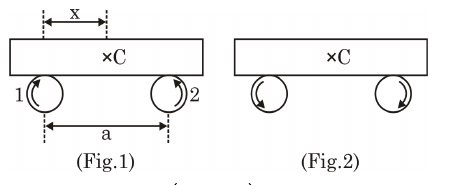
\includegraphics[width=0.95\linewidth]{Score-II - Test 44 (23 Mar 2025)-img/p1phy_q5_rollers.png}
\end{center}

(A) For case shown in fig.1
$$x(t)=\left(x_0-\dfrac a2\right)\cos\left(\sqrt{\dfrac{2\mu g}a}t\right)+\dfrac a2.$$

(B) For case shown in fig.2
$$\resizebox{\linewidth}{!}{$x(t)=\left(x_0-\dfrac a2\right)\left(\dfrac{e^{-2\omega t}+e^{2\omega t}}2\right)+\dfrac a2,\text{ where }\omega=\sqrt{\dfrac{2\mu g}a}.$}$$

(C) For case shown in fig.2
$$x(t)=\left(x_0-\dfrac a2\right)\cos\left(\sqrt{\dfrac{2\mu g}a}t\right)+\dfrac a2.$$

(D) For case shown in fig.2
$$x(t)=\left(x_0-\dfrac a2\right)\left(\dfrac{e^{\omega t}+e^{-\omega t}}2\right)+\dfrac a2,\text{ where }\omega=\sqrt{\dfrac{2\mu g}a}.$$

\textbf{6.} The figure shows electronic wave function for a hydrogen atom.

\begin{center}
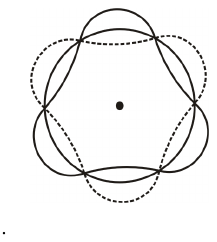
\includegraphics[width=0.5\linewidth]{Score-II - Test 44 (23 Mar 2025)-img/p1phy_q6_wavefunction.png}
\end{center}

\begin{qoptions}
\opt{A}{The quantum number of this state is 3.}
\opt{B}{The wavelength of this electron is $9\pi r_0$ (r$_0$ is radius of ground state).}
\opt{C}{H atom can go to ground state by emitting 6 different photons.}
\opt{D}{On de-excitation it is necessary that emits at least one line in infra red region of spectrum.}
\end{qoptions}

\textbf{7.} In Fig. there are two long, coaxial cylindrical shells of length $\ell$. The inner one has the radius a and the electric charge +Q, uniformly distributed over its surface. The outer cylinder has the radius b($b\ll\ell$) and the electric charge $-Q$, uniformly distributed over its surface. The cylinders are made of the same material, having the mass per unit of area equal to $\sigma$. Coaxial with them there is a long solenoid with the radius R(a $<$ R $<$ b) with n turns per unit length, and carrying and electric current i. The solenoid is fixed, but the cylindrical shells can freely and independently rotate around their common axis. Initially all the parts of this system are at rest. (Note: The cylindrical shells are heavy enough to neglect any magnetic field due to their rotation!) When current in solenoid is gradually reduced to zero. The cylinders begins to rotate. Choose the correct options:

\begin{center}
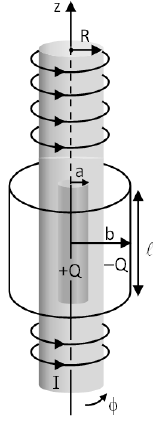
\includegraphics[width=0.4\linewidth]{Score-II - Test 44 (23 Mar 2025)-img/p1phy_q7_cylinders.png}
\end{center}

\begin{qoptions}
\opt{A}{Final angular velocity of outer cylinder is $\dfrac{\mu_0nQiR^2}{8\pi\ell\sigma b^3}$}
\opt{B}{Final angular velocity of inner cylinder is $\dfrac{\mu_0niQ}{4\pi a\sigma\ell}$}
\opt{C}{Angular momentum of the system including both cylindrical shells is conserved during the process}
\opt{D}{Angular momentum of the system consisting of two cylindrical shells is not conserved during the process}
\end{qoptions}

\subsectionhdr{Section-I (iii): Matching List Sets}

\textbf{8.} The Refractive index of lenses is 3/2. Then the final position of the image from the pole is

\end{multicols}

\begin{center}
\begin{tabular}{|c|c|c|c|}
\hline
& \textbf{List-I} & & \textbf{List-II} \\
\hline
(P) & \raisebox{-0.5\height}{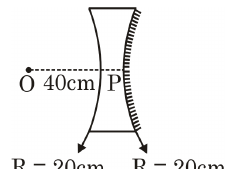
\includegraphics[width=0.22\linewidth]{Score-II - Test 44 (23 Mar 2025)-img/p1phy_q8_P.png}} & (1) & 40/7 cm, left to P \\[20pt]
\hline
(Q) & \raisebox{-0.5\height}{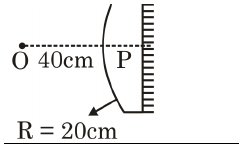
\includegraphics[width=0.22\linewidth]{Score-II - Test 44 (23 Mar 2025)-img/p1phy_q8_Q.png}} & (2) & 40/9 cm, right to P \\[20pt]
\hline
(R) & \raisebox{-0.5\height}{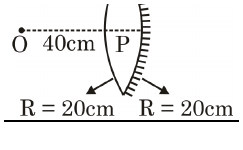
\includegraphics[width=0.22\linewidth]{Score-II - Test 44 (23 Mar 2025)-img/p1phy_q8_R.png}} & (3) & 40/3 cm, right to P \\[20pt]
\hline
(S) & \raisebox{-0.5\height}{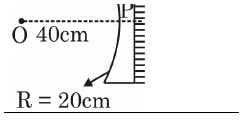
\includegraphics[width=0.22\linewidth]{Score-II - Test 44 (23 Mar 2025)-img/p1phy_q8_S.png}} & (4) & 40 cm, left to P \\[20pt]
\hline
 & & (5) & 20/3 cm, left to P \\
\hline
\end{tabular}
\end{center}

\begin{multicols}{2}
\begin{qoptions}
\opt{A}{P $\to$ 2; Q $\to$ 4; R $\to$ 1; S $\to$ 3}
\opt{B}{P $\to$ 3; Q $\to$ 1; R $\to$ 2; S $\to$ 4}
\opt{C}{P $\to$ 2; Q $\to$ 1; R $\to$ 4; S $\to$ 3}
\opt{D}{P $\to$ 2; Q $\to$ 1; R $\to$ 3; S $\to$ 4}
\end{qoptions}

\textbf{9.} A small cart with a mass m is pulled up by a light, inextensible thread. Thread is pulled at a constant speed v. Speed of cart is u at the moment. a is the acceleration of cart at the moment shown. T is the tension in the thread and P is the power developed by tension at the moment. Neglect friction. (Take m = 2 kg, v = 4 m/s, $\alpha$ = 60$^\circ$, h = 2m) (Assume cart is constrained to move horizontally by some mechanism.)

\begin{center}
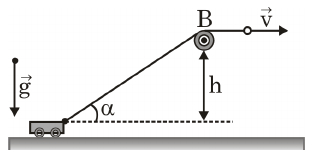
\includegraphics[width=0.85\linewidth]{Score-II - Test 44 (23 Mar 2025)-img/p1phy_q9_cart.png}
\end{center}

\begin{center}
\begin{tabular}{|c|c|c|c|}
\hline
\multicolumn{2}{|c|}{\textbf{List-I}} & \multicolumn{2}{c|}{\textbf{List-II (in SI unit)}} \\
\hline
(P) & u & (1) & 2 \\
\hline
(Q) & a & (2) & 8 \\
\hline
(R) & T & (3) & 41.52 \\
\hline
(S) & P & (4) & 664.32 \\
\hline
 & & (5) & None \\
\hline
\end{tabular}
\end{center}

\begin{qoptions}
\opt{A}{P $\to$ 2; Q $\to$ 2; R $\to$ 4; S $\to$ 5}
\opt{B}{P $\to$ 2; Q $\to$ 3; R $\to$ 5; S $\to$ 4}
\opt{C}{P $\to$ 1; Q $\to$ 3; R $\to$ 5; S $\to$ 4}
\opt{D}{P $\to$ 1; Q $\to$ 3; R $\to$ 2; S $\to$ 5}
\end{qoptions}

\textbf{10.} In the given figure, all the batteries are ideal.

\begin{center}
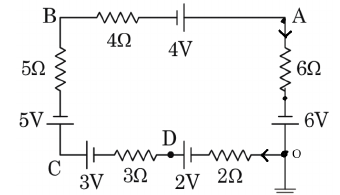
\includegraphics[width=0.85\linewidth]{Score-II - Test 44 (23 Mar 2025)-img/p1phy_q10_circuit.png}
\end{center}

\begin{center}
\begin{tabular}{|c|c|c|}
\hline
\textbf{List-I} & & \textbf{List-II} \\
\hline
(P) Potential of point A is & (1) & $-5$V \\
\hline
(Q) Potential of point B is & (2) & 1V \\
\hline
(R) Potential point C is & (3) & $-3$V \\
\hline
(S) Potential point D is & (4) & 2.5V \\
\hline
 & (5) & 0 V \\
\hline
\end{tabular}
\end{center}

\begin{qoptions}
\opt{A}{P $\to$ 1; Q $\to$ 2; R $\to$ 3; S $\to$ 4}
\opt{B}{P $\to$ 3; Q $\to$ 1; R $\to$ 2; S $\to$ 5}
\opt{C}{P $\to$ 2; Q $\to$ 3; R $\to$ 4; S $\to$ 5}
\opt{D}{P $\to$ 3; Q $\to$ 1; R $\to$ 4; S $\to$ 2}
\end{qoptions}

\textbf{11.} Box may have any series combination of L, C and R. List-I represents source current and List-II represents possible statements.

\end{multicols}

\begin{center}
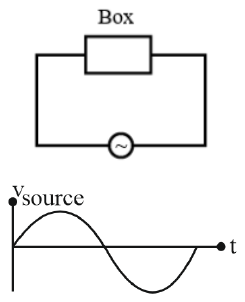
\includegraphics[width=0.25\linewidth]{Score-II - Test 44 (23 Mar 2025)-img/p1phy_q11_stem.png}
\end{center}

\begin{center}
\begin{tabular}{|c|c|c|c|}
\hline
& \textbf{List-I} & & \textbf{List-II} \\
\hline
(P) & \raisebox{-0.5\height}{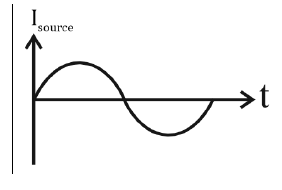
\includegraphics[width=0.22\linewidth]{Score-II - Test 44 (23 Mar 2025)-img/p1phy_q11_P.png}} & (1) & Box may contain LCR \\[20pt]
\hline
(Q) & \raisebox{-0.5\height}{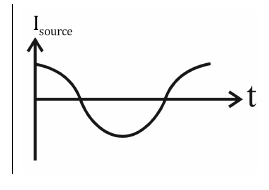
\includegraphics[width=0.22\linewidth]{Score-II - Test 44 (23 Mar 2025)-img/p1phy_q11_Q.png}} & (2) & Box may contain only LR \\[20pt]
\hline
(R) & \raisebox{-0.5\height}{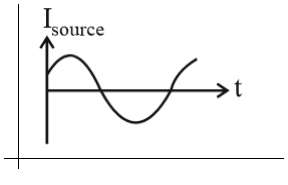
\includegraphics[width=0.22\linewidth]{Score-II - Test 44 (23 Mar 2025)-img/p1phy_q11_R.png}} & (3) & Power factor of box is zero \\[20pt]
\hline
(S) & \raisebox{-0.5\height}{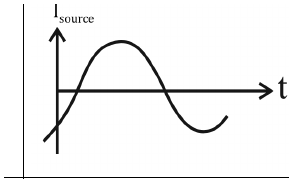
\includegraphics[width=0.22\linewidth]{Score-II - Test 44 (23 Mar 2025)-img/p1phy_q11_S.png}} & (4) & Box may contain only CR \\[20pt]
\hline
 & & (5) & State of resonance. \\
\hline
\end{tabular}
\end{center}

\begin{multicols}{2}
\begin{qoptions}
\opt{A}{P $\to$ 1,5; Q $\to$ 3; R $\to$ 4,1; S $\to$ 2,1}
\opt{B}{P $\to$ 1,5; Q $\to$ 4; R $\to$ 1; S $\to$ 5}
\opt{C}{P $\to$ 1; Q $\to$ 3; R $\to$ 4; S $\to$ 5}
\opt{D}{P $\to$ 5; Q $\to$ 5; R $\to$ 4; S $\to$ 3}
\end{qoptions}

\subsectionhdr{Section-II: Non-negative Integer}

\textbf{1.} An Ideal monatomic gas undergoes thermodynamic process (A $\to$ B), the graph of which depicted on the p $-$ V diagram in dimensionless coordinates (V/V$_0$; p/p$_0$). The work done by gas during this process is xp$_0$V$_0$. Find x.

\begin{center}
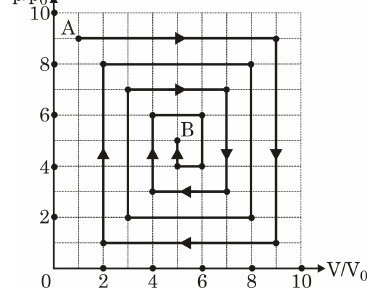
\includegraphics[width=0.85\linewidth]{Score-II - Test 44 (23 Mar 2025)-img/p1phy_n1_pvspiral.png}
\end{center}

\textbf{2.} A screw gauge is used to measure the thickness of a thin sheet of copper. The pitch of screw gauge is 0.2 mm and total number of division on circular scale is 200. When two jaws are brought in contact then $160^{th}$ division on circular scale is exactly coinciding with the main scale line, and that the zero of main scale is not visible. When thickness of sheet is measured with screw gauge then main scale reading is 0.6 mm and $100^{th}$ division coincide with the main scale line. The thickness of copper sheet is x $\times10^{-5}$ m.

\textbf{3.} A rigid rectangular frame made of thin wire can move along a smooth horizontal surface to which a thin, infinitely long straight wire is attached. The figure shows a top view of this system. Initially, the currents in the wire and in the frame are zero. The frame is at rest in such a position that one of its pairs of sides is parallel to the wire, and the distance between the wire and the side of the frame closest to it is many times greater than the entire dimensions of the frame. The current in the wire is increased to a certain maximum value so quickly that the displacement of the frame during the increase in current can be neglected. Subsequently, the current in the wire is maintained constant. It turned out that at the moment the current in the wire reaches its maximum value, the speed of the frame was equal to v$_0$. The inductance of the loop can be neglected, and its resistance can be considered constant. The frame speed is v$_0$/n after a very long time after the current in the wire reaches its maximum value. Find n.

\begin{center}
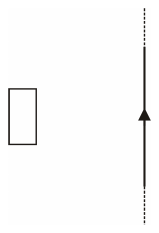
\includegraphics[width=0.35\linewidth]{Score-II - Test 44 (23 Mar 2025)-img/p1phy_n3_wireframe.png}
\end{center}

\textbf{4.} A closed organ pipe of length 99.4 cm is vibrating in its first overtone and is always in resonance with a tuning fork having variable frequency f = (300 $-$ 2t) Hz, where t is time in second. The rate by which radius of organ pipe changes when its radius is 1 cm is 1/N m/s then find N. (speed of sound in organ pipe = 320 m/s)

\textbf{5.} The distance between a screen and a light source lined up on an optical bench is 120 cm. When a lens is moved along the line joining them, sharp images of the source can be obtained at two lens positions; the size ratio of these two images is 1 : 9. Write value of $2\times$ focal length (in cm)

\textbf{6.} Boron atoms of mass number A = 10 and a beam of unidentified particles, moving in opposite directions with the same (non-relativistic) speed, are made to collide inside an ion accelerator. The maximum scattering angle of the boron atoms is found to be 30$^\circ$. What is the atomic mass number of ion. (Assume elastic collision)

\sectionhdr{PART-2: CHEMISTRY}
\subsectionhdr{Section-I (i): Single Correct}

\textbf{1.}

\begin{center}
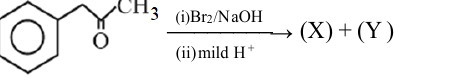
\includegraphics[width=0.85\linewidth]{Score-II - Test 44 (23 Mar 2025)-img/p2chem_q1_reaction.png}
\end{center}

Given: molar mass of 'X' is greater than 'Y'

'X' and 'Y' are considered as major products

Identify the \textbf{INCORRECT} statement?

\begin{qoptions}
\opt{A}{'X' and 'Y' can be differentiated by NaHCO$_3$ aqeuous solution}
\opt{B}{At room temperature, 'X' is a colourless solid and 'Y' is a colourless liquid}
\opt{C}{Acidic strength: X $>$ Y}
\opt{D}{'Y' can be used to prepare non-essential amino acid}
\end{qoptions}

\textbf{2.} In the following statements

(i) When a freshly prepared precipitate of SnO$_2$ is peptized by small amount of NaOH, then a negative sol is formed.

(ii) Coagulation is an irreversible process.

(iii) Brownian motion stabilizes while electrical double layer distabilizes the colloidal solution

(iv) Micelle formation is an entropy driven process.

The \textbf{CORRECT} statements are

\begin{qoptions}
\opt{A}{(i), (ii), (iv) only}
\opt{B}{(i), (ii), (iii), (iv)}
\opt{C}{(i), (iv)}
\opt{D}{(iv) only}
\end{qoptions}

\textbf{3.} A vessel contains three ideal gases: w$_1$ gm He, w$_2$ gm CH$_4$ and w$_3$ gm SO$_2$. Find the ratio [w$_1$ : w$_2$ : w$_3$], if these three gases effuse out of an orifine in the vessel in equal volume ratio? [Atomic mass: He = 4, S = 32]

\begin{qoptions}
\opt{A}{1 : 4 : 16}
\opt{B}{1 : 8 : 32}
\opt{C}{1 : 8 : 64}
\opt{D}{1 : 4 : 32}
\end{qoptions}

\textbf{4.} Which one of the following statement is \textbf{INCORRECT} regarding Ziese's salt

\begin{qoptions}
\opt{A}{IUPAC name is Potas\-si\-um tri\-chlo\-ri\-do(di\-hap\-to\-eth\-yl\-ene)pla\-ti\-nate(II)}
\opt{B}{Contains two different Pt$-$C$\ell$ bond lengths}
\opt{C}{All four hydrogens and two carbons of ethylene ligand are present in same plane}
\opt{D}{C-C bond length in Ziese'e salt is less than that is K[PtC$\ell_3$(C$_2$F$_4$)]}
\end{qoptions}

\subsectionhdr{Section-I (ii): One or more correct}

\textbf{5.}

\begin{center}
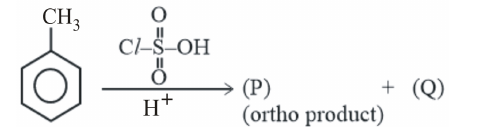
\includegraphics[width=0.85\linewidth]{Score-II - Test 44 (23 Mar 2025)-img/p2chem_q5_stem.png}
\end{center}

(P) $\xrightarrow{\text{NH}_3}$ (R) $\xrightarrow[\text{(ii) mild H}^+]{\text{(i) KMnO}_4/\text{OH}^-,\Delta}$ (S) $\xrightarrow[\Delta]{\text{conc.H}^+}$ (T)

Given: (P) and (Q) are isomers

Identify the \textbf{CORRECT} statement(s)

\begin{qoptions}
\opt{A}{Sodium fusion extract of 'T' gives blood red solution with neutral FeC$\ell_3$ solution}
\opt{B}{\raisebox{-0.4\height}{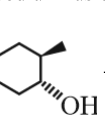
\includegraphics[width=0.25\linewidth]{Score-II - Test 44 (23 Mar 2025)-img/p2chem_q5_optB.png}}\ $\xrightarrow[\text{(ii) (CH}_3\text{)}_2\text{CuLi/ether}]{\text{(i) (Q)/Pyridene}}$ (U). Then, 'U' is a meso product}
\opt{C}{'T' can be used for masking the bitter taste of some medicines in pharmaceutical industry}
\opt{D}{Sodium salt of 'T' is used in many foods as non-nutritive sweetener}
\end{qoptions}

\textbf{6.} n$-$Hexane $\xrightarrow[\text{At High T,P}]{\text{A}\ell_2\text{O}_3/\text{Cr}_2\text{O}_3}$ (P) $\xrightarrow[\Delta]{\text{oleum}}$ (Q) $\xrightarrow[\text{(ii) mild H}^+]{\text{(i) Fused NaOH}/\Delta}$ (R) $\xrightarrow{\text{K}_2\text{S}_2\text{O}_8/\text{dil. OH}^-}$ (S)

Which of the following is/are \textbf{CORRECT}?

\begin{qoptions}
\opt{A}{Alkaline solution of (S) is used in developing of unexposed photographic film into negative}
\opt{B}{(R) gives violet colour solution with neutral FeC$\ell_3$ solution}
\opt{C}{(Q) changes to (P), when it is heated with dil. H$^+$}
\opt{D}{(P) and (R) can be distinguished by using Br$_2$/H$_2$O}
\end{qoptions}

\textbf{7.} 0.1 mole AgNO$_3$ is added in 250m$\ell$ of saturated solution of AgC$\ell$ at 25$^\circ$C without changing the volume of solution.

Given: K$_{SP}$ of AgC$\ell$ $=1.0\times10^{-10}$ M$^2$ at 25$^\circ$C

Limiting molar conductance of Ag$^+$ ion $=60\ \Omega^{-1}$cm$^2$mol$^{-1}$

Limiting molar conductance of C$\ell^-$ ion $=75\ \Omega^{-1}$cm$^2$mol$^{-1}$

Limiting molar conductance of NO$_3^-$ ion $=75\ \Omega^{-1}$cm$^2$mol$^{-1}$

Which of the following statement(s) is/are \textbf{CORRECT}?

\begin{qoptions}
\opt{A}{O$_2$ gas is liberated at anode, if this solution is electrolysed by using inert electrodes}
\opt{B}{Total conductivity of this solution $\approx5.4\times10^{-2}\ \Omega^{-1}$cm$^{-1}$}
\opt{C}{Concentration of C$\ell^-$ in resulting solution is $2.5\times10^{-9}$ M}
\opt{D}{In the final solution, concentration of Ag$^+$ is 0.4 M}
\end{qoptions}

\subsectionhdr{Section-I (iii): Matching List Sets}

\textbf{8.} Match the possible combinations for COMPOUNDS in List-I and REAGENTS used in their differentiating tests in List-II

\end{multicols}

\begin{center}
\begin{tabular}{|c|l|c|l|}
\hline
& \textbf{List-I (compounds)} & & \textbf{List-II (Reagents)} \\
\hline
(P) & Glucose and sucrose & (1) & Resorcinol under acidic medium \\
\hline
(Q) & Glucose and fructose & (2) & Alkaline CuSO$_4$ and tartrate ion \\
\hline
(R) & Butanone and acetyl chloride & (3) & AgNO$_{3(aq)}$ / $\Delta$ \\
\hline
(S) & Phenol and Benzoic acid & (4) & NaHCO$_{3(aq)}$ \\
\hline
 & & (5) & Resultant of (HI+HIO$_3$) then NaOH \\
\hline
\end{tabular}
\end{center}

\begin{multicols}{2}
\begin{qoptions}
\opt{A}{P $\to$ 1; Q $\to$ 2; R $\to$ 3; S $\to$ 4}
\opt{B}{P $\to$ 2; Q $\to$ 1; R $\to$ 3,5; S $\to$ 4}
\opt{C}{P $\to$ 1,5; Q $\to$ 2,4; R $\to$ 5; S $\to$ 4}
\opt{D}{P $\to$ 2; Q $\to$ 1,4; R $\to$ 3,5; S $\to$ 2,3}
\end{qoptions}

\textbf{9.} Select the correct match of List I with List II about FCC(ABCABC...) packing, where 'a' is the edge length of unit cell.

\end{multicols}

\begin{center}
\begin{tabular}{|l|c|c|}
\hline
\textbf{List-I} & \multicolumn{2}{c|}{\textbf{List-II}} \\
\hline
(P) Nearest distance between nearest octahedral and tetrahedral void & (1) & $\dfrac a{\sqrt2}$ \\[6pt]
\hline
(Q) Nearest distance between two nearest octahedral voids & (2) & $\dfrac a2$ \\[6pt]
\hline
(R) Nearest distance between two nearest tetrahedral voids & (3) & $\dfrac{\sqrt3a}4$ \\[6pt]
\hline
(S) Nearest distance between layers A and B & (4) & $\dfrac a{\sqrt3}$ \\[6pt]
\hline
 & (5) & $\dfrac a{2\sqrt3}$ \\[6pt]
\hline
\end{tabular}
\end{center}

\begin{multicols}{2}
\begin{qoptions}
\opt{A}{P $\to$ 3; Q $\to$ 2; R $\to$ 4; S $\to$ 1}
\opt{B}{P $\to$ 3; Q $\to$ 1; R $\to$ 2; S $\to$ 4}
\opt{C}{P $\to$ 1; Q $\to$ 2; R $\to$ 3; S $\to$ 4}
\opt{D}{P $\to$ 2; Q $\to$ 3; R $\to$ 4; S $\to$ 1}
\end{qoptions}

\textbf{10.} Match the polymers in List-I with their characteristic in List-II and choose the correct option from the codes given below:

\begin{center}
\begin{tabular}{|c|l|c|l|}
\hline
\multicolumn{2}{|c|}{\textbf{List-I}} & \multicolumn{2}{c|}{\textbf{List-II}} \\
\hline
(P) & Bakelite & (1) & Natural polymer \\
\hline
(Q) & Natural rubber & (2) & Addition polymer \\
\hline
(R) & Buna-N & (3) & Linear polymer \\
\hline
(S) & Cellulose & (4) & Co-polymer \\
\hline
 & & (5) & Thermosetting plastic \\
\hline
\end{tabular}
\end{center}

\begin{qoptions}
\opt{A}{P $\to$ 4,5; Q $\to$ 1,2,3; R $\to$ 2,3,4; S $\to$ 1,3}
\opt{B}{P $\to$ 1,2; Q $\to$ 4,5; R $\to$ 2,3,4; S $\to$ 1,3}
\opt{C}{P $\to$ 4,5; Q $\to$ 2,3,4; R $\to$ 1,2,3; S $\to$ 2,4}
\opt{D}{P $\to$ 1,4; Q $\to$ 1,2; R $\to$ 2,3; S $\to$ 3,4}
\end{qoptions}

\textbf{11.} Match the following metal given in List-I with the appropriate metal extraction process listed with List-II

\begin{center}
\begin{tabular}{|c|l|c|l|}
\hline
\multicolumn{2}{|c|}{\textbf{List-I}} & \multicolumn{2}{c|}{\textbf{List-II}} \\
\hline
(P) & Fe & (1) & Cyanide Process \\
\hline
(Q) & Ag & (2) & Leaching \\
\hline
(R) & Pb & (3) & Carbon reduction \\
\hline
(S) & Cu & (4) & Self reduction \\
\hline
 & & (5) & Electrolysis \\
\hline
\end{tabular}
\end{center}

\begin{qoptions}
\opt{A}{P $\to$ 3; Q $\to$ 2,3; R $\to$ 4,5; S $\to$ 4,5}
\opt{B}{P $\to$ 3,5; Q $\to$ 1,2,3,5; R $\to$ 3,5; S $\to$ 4,5}
\opt{C}{P $\to$ 3; Q $\to$ 1,2,5; R $\to$ 3,4,5; S $\to$ 2,4,5}
\opt{D}{P $\to$ 2,3; Q $\to$ 1,2,3,4,5; R $\to$ 1,2,4,5; S $\to$ 2,5}
\end{qoptions}

\subsectionhdr{Section-II: Non-negative Integer}

\textbf{1.} A colourless inorganic salt(A) decomposes completely at above 250$^\circ$C to give only neutral, diamagnetic gaseous products(B) and (C) leaving no residue. The oxide(C) is a liquid at room temperature and gas 'B' is a supporter of combustion. White P$_4$ burns in excess of 'B' to produce a strong dehydrating agent(D).

(B) $\xrightarrow{\text{NaNH}_2}$ (P)$\uparrow$ + (Q) + (R) \quad [salt]

Determine the maximum amount of NaNH$_2$ in gram to produce one mole of 'P'

Given: 'P' is a colourless and pungent smell gas

'Q' is used in car air bags

'R' turns red litmus to blue

Atomic mass: Na-23, N-14, H-1, O-16, P-31

\textbf{2.} For a gas phase reaction: A$_{(g)}\rightleftharpoons$B$_{(g)}$, gas A is 80\% dissociated at equilibrium at 10 bar and 227$^\circ$C. Calculate $|\Delta_rG^\circ|$ for the reaction (in cal/mol)?

Given: Rate constant of forward reaction is $0.693\times10^{-3}\ \text{sec}^{-1}$ and $\ell n(2)=0.693$

\textbf{3.} Chromite ore $\xrightarrow[\text{(Fusion)}]{\text{Na}_2\text{O}_2}$ (P) + (Q) $\xrightarrow[\text{(ii) Filter}]{\text{(i) excess of H}_2\text{O}/\Delta}$ Filtrate (P) $\xrightarrow[\text{(ii) Evaporation}]{\text{(i) CO}_2\text{(g)}}$ Solid (R)

In the following statements

(i) (Q) can be used to oxidize impurities present in cast iron/pig iron to produce wrought iron

(ii) `A$\ell$' reduction method can be used in the commercial extraction of metal present in (Q)

(iii) Aqueous solution of (R) can be used as primary standard solution in the quantitative estimation of Mohr's salt

(iv) (P) to (R) conversion involves redox change

(v) Yellow colour solution of (P) involves metal to ligand charge transfer

(vi) n-factor of chromite in the reaction with fused Na$_2$O$_2$ is 7

(vii) Crystals of (R) gives diamagnetic gas with conc. HC$\ell$/$\Delta$

(viii) Oxidising power: (P) $>$ (R)

Find the value of (Y$-$X)

If

X = Number of CORRECT statements

Y = Number of INCORRECT statements

\textbf{4.} MgC$\ell_{2(aq)}$ $\xrightarrow[\text{NH}_4\text{C}\ell/\text{NH}_4\text{OH}]{\text{NaH}_2\text{PO}_4}$ (X)$\downarrow$ $\xrightarrow\Delta$ (Y)$\downarrow$ + other products \quad [(X): white ppt, (Y): white ppt]

Determine P$^{(\text{solubility of X})}$ at pH=10 and 25$^\circ$C. (Answer to the nearest integer)

Given: 'P' means $(-\log_{10})$

At equilibrium, $[\text{NH}_4^+]=0.01$M

K$_{sp}$(X) $=10^{-12}$ at 25$^\circ$C

For H$_3$PO$_4$: P$^{ka_1}=3$, P$^{ka_2}=7$, P$^{ka_3}=12$

\textbf{5.} Tetrasaccharide of D-mannose is obtained by C$_1$-C$_4$ glycosidic linkage between successive pyranose form of D-mannose. Determine total number of possible tetrasaccharides can be obtained

\textbf{6.} C$_4$H$_{10}$O(Z) $\xrightarrow{\text O_2}$ (P) + (Q) $\xrightarrow[\text{(ii) KSCN(aq)}]{\text{(i) FeSO}_4\text{(aq)}}$ (R) [coloured solution] $\xrightarrow[\text{(excess)}]{\text{KF}_{(aq)}}$ (S) [colourless solution]

'Z' is a volatile compound and its is insoluble in NaOH

If

The theoretical spin-only magnetic moment of (R) = 'X' BM

E.A.N value of 'S' = 'Y'

Then, the value (Y$-$X) is (nearest integer)

\sectionhdr{PART-3: MATHEMATICS}
\subsectionhdr{Section-I (i): Single Correct}

\textbf{1.} Consider polynomials P(x) of degree at most 3, each of whose coefficients is an element of $\{0,1,2,3,4,5,6,7,8,9,10,11\}$. How many such polynomials satisfy P($-1$) $=-11$?

\begin{qoptions}
\opt{A}{286}
\opt{B}{364}
\opt{C}{336}
\opt{D}{220}
\end{qoptions}

\textbf{2.} If $\displaystyle\prod_{r=0}^{89}\left(a+b\omega^r+c\omega^{2r}\right)=\begin{vmatrix}a&b&c\\b&c&a\\c&a&b\end{vmatrix}^k$; then k is equal to (where $\omega$ is the complex (non real) cube root of unity and a,b,c$\in\mathbb R$)

\begin{qoptions}
\opt{A}{20}
\opt{B}{30}
\opt{C}{21}
\opt{D}{31}
\end{qoptions}

\textbf{3.} If $\sin^{-1}x+\cos^{-1}x+\tan^{-1}\dfrac1x+\tan^{-1}x=\pi k$. The value of k for different values of x are k$_1$ and k$_2$, satisfying the equations $\dfrac{x^2}{4k_1}+\dfrac{y^2}5=1$ and $y^2=12(x-k_2)$, then the equation of their common tangent is

\begin{qoptions}
\opt{A}{$y=2x-5$}
\opt{B}{$3y=x+3$}
\opt{C}{$y=x+3$}
\opt{D}{$y=3x+1$}
\end{qoptions}

\textbf{4.} Let A(m) denotes the area of the region bounded by the curve $y=2^{2^{x+x-2}}\cdot(\ln2)^2$ and x-axis between the lines x = 1 and x = m (m$\in\mathbb N$, m $>$ 2), then A(m) + 2 is

\begin{qoptions}
\opt{A}{A prime number for all m}
\opt{B}{A composite number for all m}
\opt{C}{A prime number for some m}
\opt{D}{An irrational number for some m}
\end{qoptions}

\subsectionhdr{Section-I (ii): One or more correct}

\textbf{5.} Let M = $[a_{ij}]_{3\times2}$ and N = $[b_{ij}]_{2\times3}$ be two matrices such that MN $=\begin{bmatrix}8&2&-2\\2&5&4\\-2&4&5\end{bmatrix}$ \& det(NM) $\ne0$, then choose the correct option(s) (P is a $2\times2$ matrix)

\begin{qoptions}
\opt{A}{Det(NM) = 81}
\opt{B}{If P(NM) = I, then $\displaystyle\lim_{n\to\infty}\det\left(P+P^2+\cdots+P^n\right)=\dfrac1{16}$}
\opt{C}{det(NM) = 9}
\opt{D}{If P(NM) = I, then $\displaystyle\lim_{n\to\infty}\det\left(P+P^2+\cdots+P^n\right)=\dfrac1{64}$}
\end{qoptions}

\textbf{6.} Let S(a$_1$, r) denote the geometric progression with first term a$_1$ and common ratio r such that a$_1\in\mathbb N$ and r$\in\mathbb Q-\{0\}$ and a$_1+a_2+a_3=19$ where a$_k$ denotes k$^{th}$ term of G.P (geometric progression). Let F be the set of all such G.P's defined above. Then TRUE statements is/are (NOTE: N and Q represents set of natural and rational numbers respectively)

\begin{qoptions}
\opt{A}{F contains 7 such G.P}
\opt{B}{F contains 4 such G.P}
\opt{C}{In all such possible G.P difference of maximum \& minimum common ratio is 4}
\opt{D}{There exist some S(a$_1$, r) $\in$ F such that a$_1$a$_4$ = 24}
\end{qoptions}

\textbf{7.} P(x) is a fourth degree polynomial such that

(1) P($-$x) = P(x) $\forall$ x $\in$ R,

(2) P(x) $>$ 0 $\forall$ x $\in$ R,

(3) P(0) = 1,

(4) P(x) has exactly two local minima at x$_1$ and x$_2$ such that $|x_1-x_2|=2$.

The line y = 1 touches the curve at a certain point Q and the enclosed area between the line and the curve is $\dfrac{8\sqrt2}{15}$. Let g(x) $=Ax^2+Bx+C$ (A $\ne$ 0) such that $\displaystyle\lim_{x\to0}\dfrac{P(x)-g(x)-g(-x)}{x^2}$ is finite and is equal to the slope of the tangent of g(x) at x $=-1$. If y = 1 is also a tangent to g(x), then

\begin{qoptions}
\opt{A}{The value of A is $-\dfrac12$}
\opt{B}{The value of B + C is $-\dfrac12$}
\opt{C}{The value of A + C is 1}
\opt{D}{The value of A + B + C is $-1$}
\end{qoptions}

\subsectionhdr{Section-I (iii): Matching List Sets}

\textbf{8.} Let $S=\{(a,b,c)\in\mathbb R^3:|ax+by+cz|+|bx+cy+az|+|cx+ay+bz|=|x|+|y|+|z|$; for all real numbers x, y and z$\}$ (Note: $|x|$ is absolute value function) Match each entry in List-I to the correct entries in List-II.

\end{multicols}

\begin{center}
\begin{tabular}{|c|l|c|l|}
\hline
\multicolumn{2}{|c|}{\textbf{List-I}} & \multicolumn{2}{c|}{\textbf{List-II}} \\
\hline
(P) & $\displaystyle\sum_{(a,b,c)\in S}|a|$ & (1) & 0 \\[8pt]
\hline
(Q) & $\displaystyle\sum_{(a,b,c)\in S}|b|$ & (2) & 1 \\[8pt]
\hline
(R) & $\displaystyle\sum_{(a,b,c)\in S}|a||b||c|$ & (3) & 2 \\[8pt]
\hline
(S) & $\displaystyle\sum_{(a,b,c)\in S}(a^2+b^2+c^2)$ & (4) & 3 \\[8pt]
\hline
& & (5) & 6 \\
\hline
\end{tabular}
\end{center}

\begin{multicols}{2}
Then correct option is

\begin{qoptions}
\opt{A}{P $\to$ 4; Q $\to$ 4; R $\to$ 2; S $\to$ 5}
\opt{B}{P $\to$ 4; Q $\to$ 4; R $\to$ 1; S $\to$ 5}
\opt{C}{P $\to$ 3; Q $\to$ 3; R $\to$ 1; S $\to$ 5}
\opt{D}{P $\to$ 3; Q $\to$ 1; R $\to$ 3; S $\to$ 4}
\end{qoptions}

\textbf{9.} Consider functions f$_i$: $\mathbb R\to\mathbb R$ for i = 1, 2, 3 as
$$f_1(x)=\dfrac{7x}8+\dfrac12\int_0^1xt\left(f_1^2(t)\right)dt$$
$$f_2(x)=1+\dfrac2\pi\int_0^\pi\cos^2x(f_2(t))dt$$
$$f_3(x)=x+\int_0^1xt(f_3(t))dt$$
Denote $\|f_i\|$ as number of differentiable functions satisfying the above integral equation. Then Match each entry in List-I to the correct entries in List-II

\end{multicols}

\begin{center}
\begin{tabular}{|c|l|c|l|}
\hline
\multicolumn{2}{|c|}{\textbf{List-I}} & \multicolumn{2}{c|}{\textbf{List-II}} \\
\hline
(P) & $\|f_1(x)\|$ & (1) & 0 \\
\hline
(Q) & $\|f_2(x)\|$ & (2) & 1 \\
\hline
(R) & $\|f_3(x)\|$ & (3) & 2 \\
\hline
(S) & Value of f$_1(0)$ + f$_3(2)$ & (4) & 3 \\
\hline
 & & (5) & 4 \\
\hline
\end{tabular}
\end{center}

\begin{multicols}{2}
The correct option is

\begin{qoptions}
\opt{A}{P $\to$ 3; Q $\to$ 4; R $\to$ 1; S $\to$ 5}
\opt{B}{P $\to$ 2; Q $\to$ 1; R $\to$ 4; S $\to$ 3}
\opt{C}{P $\to$ 3; Q $\to$ 1; R $\to$ 2; S $\to$ 4}
\opt{D}{P $\to$ 2; Q $\to$ 1; R $\to$ 3; S $\to$ 4}
\end{qoptions}

\textbf{10.} Answer the following by appropriately matching the lists based on the information given in the paragraph. Consider the planes

P$_1$: x + y $-$ z = 5

P$_2$: 2x $-$ y + $\lambda$z = 3 (where $\lambda\in\mathbb R$)

P$_3$: x $-$ 3y $-$ 4 = 0

P$_4$: 4y $-$ z + 5 = 0

Plane P$_1$ and P$_2$ intersect to form line L$_1$. Plane P$_3$ and P$_4$ intersect to form line L$_2$. There are some expression given in the List-I match them with the List-II given below.

\end{multicols}

\begin{center}
\begin{tabular}{|c|l|c|l|}
\hline
\multicolumn{2}{|c|}{\textbf{List-I}} & \multicolumn{2}{c|}{\textbf{List-II}} \\
\hline
(P) & Value of $\lambda$ for which L$_1$ and L$_2$ are coplanar & (1) & $-\dfrac54$ \\[8pt]
\hline
(Q) & Image of the line L$_2$ in the plane P$_1$ is passing through & (2) & $(0,-33,0)$ \\
\hline
(R) & Image of plane P$_1$ in the plane P$_3$ is passing through & (3) & $-\dfrac65$ \\[8pt]
\hline
(S) & Equation of the line L$_2$ is passing through & (4) & $(1,-1,1)$ \\
\hline
 & & (5) & $(-1,1,-11)$ \\
\hline
\end{tabular}
\end{center}

\begin{multicols}{2}
The correct option is

\begin{qoptions}
\opt{A}{P $\to$ 1; Q $\to$ 5; R $\to$ 2; S $\to$ 4}
\opt{B}{P $\to$ 3; Q $\to$ 4; R $\to$ 2; S $\to$ 5}
\opt{C}{P $\to$ 3; Q $\to$ 5; R $\to$ 2; S $\to$ 4}
\opt{D}{P $\to$ 1; Q $\to$ 4; R $\to$ 2; S $\to$ 5}
\end{qoptions}

\textbf{11.} Let $f(x)=\displaystyle\lim_{n\to\infty}\prod_{k=0}^{n-1}\dfrac{\left(x^{2^k}+1\right)^2}{\left(x^{2^{k+1}}+1\right)}\ \forall x\in[0,\infty)-\{1\}$ \& f(1) = 1, then there are some expression given in the List-I match them with the List-II given below

\end{multicols}

\begin{center}
\begin{tabular}{|c|l|c|l|}
\hline
\multicolumn{2}{|c|}{\textbf{List-I}} & \multicolumn{2}{c|}{\textbf{List-II}} \\
\hline
(P) & f(x) is increasing in & (1) & $x\in(1,\infty)$ \\
\hline
(Q) & f(x) is decreasing in & (2) & $x\in\left(0,\dfrac12\right)\cup(5,\infty)$ \\[8pt]
\hline
(R) & f(x) has a local minima in & (3) & $x\in(0,1)$ \\
\hline
(S) & f(x) = x has only one solution in & (4) & $x\in(0,2)$ \\
\hline
 & & (5) & $x\in(0,1)\cup(4,5)$ \\
\hline
\end{tabular}
\end{center}

\begin{multicols}{2}
The correct option is

\begin{qoptions}
\opt{A}{P $\to$ 3; Q $\to$ 4; R $\to$ 1; S $\to$ 5}
\opt{B}{P $\to$ 2; Q $\to$ 1; R $\to$ 4; S $\to$ 3}
\opt{C}{P $\to$ 3; Q $\to$ 1; R $\to$ 4; S $\to$ 4}
\opt{D}{P $\to$ 2; Q $\to$ 1; R $\to$ 3; S $\to$ 4}
\end{qoptions}

\subsectionhdr{Section-II: Non-negative Integer}

\textbf{1.} Let a, b, c, d, e $\in[-2,2]$, such that $\sum a=0$, $\sum a^3=0$, $\sum a^5=10$. If a $\ge$ b $\ge$ c $\ge$ d $\ge$ e, find the value of $a^2+bd-ce$.

\textbf{2.} Consider a line L: $\dfrac x{2024}+\dfrac y{2025}=1$

Let F be the family of circles tangent to line L and also tangent to lines given by xy = 0 (coordinate axes). If C$_1$, C$_2$, C$_3$, \ldots\ldots\ldots, C$_n\in$F with radius $r_1<r_2<\ldots\ldots<r_n$.

Then $|r_1+r_2+r_3-r_4|$ equals \ldots\ldots\ldots

\textbf{3.} A fair six-sided dice has `1' on one face, `2' on two of its faces, `3', on the remaining 3 faces. The die is thrown twice and X is the random variable `total score thrown'. The mean of the variable Y $=|X^2-6X|$ is A and Var(X) $+(E(X))^2$ = B. Then [A] + [B] is (Note: [x] is greatest integer function and all symbols have usual meaning)

\textbf{4.} Using the identity $\dfrac1{^{2n+1}C_r}+\dfrac1{^{2n+1}C_{r+1}}=\dfrac{2n+2}{2n+1}\cdot\dfrac1{^{2n}C_r}$

$A_n=\dfrac{6(n+2)}n\displaystyle\sum_{r=1}^{n-1}\dfrac{(-1)^{r-1}r}{^nC_r}$

$B_n=\displaystyle\sum_{r=n-100}^{n-1}(-1)^r\ ^nC_r$ for n $\ge100$

\&

$C=\displaystyle\sum_{r=0}^{100}\ ^{1012}C_r\cdot\ ^{1011}C_{100-r}$, then value of $A_{2024}-B_{2024}+C$ is

\textbf{5.} A line touches a hyperbola at P and intersects the pair of asymptotes at point Q and R. If equation of pair of asymptotes is given by $4x^2+8xy-y^2=0$ and mid-point of QR is (1, 0). If circumcenter of $\triangle$OQR is (a, b) then value of a $-$ b is

\textbf{6.} $f(x)=\displaystyle\prod_{k=1}^\infty\left(\dfrac{1+2\cos\left(\dfrac{2x}{3^k}\right)}3\right)$, then number of points where $[xf(x)]+|xf(x)|+(x-1)|x^2-3x+2|$ is non-differentiable in x$\in(0,3\pi)$ is equal to (where [.] denotes greatest integer function)

\end{multicols}
\end{document}
